\documentclass[12pt]{article}
\input{etc/cmd}
\usepackage{amsmath}
\usepackage{amsfonts}
\usepackage{amssymb}
\begin{document}
\fontsize{12pt}{14pt}\selectfont

\begin{minipage}{0.1\textwidth}
    \includegraphics[width=2cm]{etc/sut}
    \end{minipage}%
    %\hfill%
    \hspace{1.65cm}
    \begin{minipage}{0.5\textwidth}\centering
    \fontsize{10pt}{10pt}\selectfont
    به‌نام خدا \\
    تئوری یادگیری ماشین \\
    دکتر سیدصالحی \\
    جلسه چهاردهم \\
    \vspace{0.25cm}
    \begingroup
    \fontsize{8pt}{8pt}\selectfont
    دانشکده ریاضی و علوم کامپیوتر \\
    اردیبهشت ماه ۱۴۰۳ \\
    \endgroup
    \end{minipage}%
    \hfill%
    \begin{minipage}{0.1\textwidth}
    %\includegraphics[width=1.8cm]{etc/ce}
    \end{minipage}
    
    \vspace{0.5cm}
    
    \noindent\rule{\textwidth}{1pt}
    
\section{ ماشین های بردار پشتیبان}
$SVM$
یک الگوریتم یادگیری ماشین نظارت شده است که برای وظایف طبقه‌بندی و رگرسیون استفاده می‌شود. این فصل چندین مفهوم کلیدی و فرمول‌بندی‌های مرتبط با $SVM$
‌ها را تشریح می‌کند.
ابتدا مثالی از مسئله بهینه سازی سر کلاس دیدیم . 
ما داستان ماشین‌های بردار پشتیبان
$SVMs$ را با صحبت درباره حاشیه‌ها
آغاز می‌کنیم.
این بخش، بینشی درباره حاشیه‌ها و درباره «اطمینان»
پیش‌بینی‌های
ما خواهد داد.
میخواهیم خطی را پیدا کنیم که احتمالا در آینده قدرت 
تعمیم%
\LTRfootnote{generalization}
بیشتری خواهد داشت ، ذدر این مرحله 
حاشیه%
\LTRfootnote{margin} 
داریم و هدف ما 
بیشینه کردن 
حاشیه  
یا به نوعی بیشترین حاشیه است . 
در ادامه شهود ما نسبت به بیشینه سازی حاشیه و شرط خود را نوشتیم .
مسئله ی 
محدب %
\LTRfootnote{convex} 
ما یک جواب دارد که به این نوع مسائل 
ماشین های بردار پشتیبان حاشیه سخت %
\LTRfootnote{hard margin svm} 
گفته می شود .


\subsection*{فهرست}
\begin{enumerate}
  \item مفهوم حاشیه
  \item $SVM$ حاشیه سخت
  \item مسئله دوگانه $SVM$ حاشیه سخت
  \item $SVM$ حاشیه نرم
  \item مسئله دوگانه $SVM$ حاشیه نرم
\end{enumerate}
\subsection{مفهوم حاشیه}
حاشیه یک صفحه‌ی تصمیم که نمونه‌های دو کلاس قابل تفکیک خطی را جدا می‌کند، کوچکترین فاصله بین مرز تصمیم و هر یک از نمونه‌های آموزشی است. حاشیه بزرگتر معمولاً بهتر به داده‌های دیده نشده تعمیم می‌یابد.

\section{
فرمولاسیون دوگانه
}
%
\LTRfootnote{Dual formulation of the SVM}

فرمولاسیون دوگانه ماشین بردار پشتیبان $SVM$ یک روش جایگزین برای حل مسئله اصلی اولیه است. این فرمولاسیون بینش بیشتری به 
ابرصفحه %
\LTRfootnote{hyper-plane}
بهینه می دهد و استفاده از ترفند کرنل را امکان پذیر می کند.


\subsection{
تکنیک ضرایب لاگرانژ
}
فرمولاسیون دوگانه بر اساس تکنیک مولتی پلیر لاگرانژ است، که یک روش بهینه سازی برای حل مشکلات با محدودیت های مساوی یا نا مساوی است. این تکنیک شامل معرفی متغیرهای جدید به نام مولتی پلیر لاگرانژ است که مسئله بهینه سازی محدود را به یک مسئله بهینه سازی بدون محدودیت تبدیل می کند.
\subsection{مزایای کلیدی}

فرمولاسیون دوگانه 
\lr{SVM}
چندین مزیت را ارائه می دهد، از جمله:
\begin{itemize}
\singlespace
    \item بینش بیشتری به ابرصفحه بهینه می دهد
    \item 
استفاده از ترفند کرنل را امکان پذیر می کند که برای طبقه بندی غیر خطی استفاده می شود
    \item
یک راه حل جایگزین برای مسئله اصلی اولیه را ارائه می دهد که در برخی از موقعیت ها مفید است.

\end{itemize}

\subsection*{حاشیه سخت}
مسئله بهینه‌سازی: هدف یافتن یک صفحه‌ی تصمیم است که حاشیه بین دو کلاس را به حداکثر برساند.
\begin{latin}
    
\begin{align*}
  \text{max}_{M,\mathbf{w},w_0} \frac{2M}{||\mathbf{w}||} \\
  \text{subject to} \\
  y_i (\mathbf{w}^T \mathbf{x}_i + w_0) \geq M \quad \forall i
\end{align*}
\end{latin}
تغییر مقیاس پارامترها: این مسئله بهینه‌سازی را با ثابت کردن حاشیه به 1 ساده می‌کند.
\begin{latin}
    \begin{align*}
  \text{max}_{\mathbf{w}',w_0'} \frac{2}{||\mathbf{w}'||} \\
  \text{subject to} \\
  y_i (\mathbf{w}'^T \mathbf{x}_i + w_0') \geq 1 \quad \forall i
\end{align*}
\end{latin}

فرمول‌بندی معادل:
\begin{latin}
    \begin{align*}
  \text{min}_{\mathbf{w},w_0} \frac{1}{2} ||\mathbf{w}||^2 \\
  \text{subject to} \\
  y_i (\mathbf{w}^T \mathbf{x}_i + w_0) \geq 1 \quad \forall i
\end{align*}
\end{latin}

\subsection*{فرمول‌بندی دوگانه $SVM$ حاشیه سخت}
تکنیک ضرایب لاگرانژ: برای مسائل با محدودیت‌های برابری یا نابرابری مفید است.

\begin{latin}
    \[
    \begin{aligned}
        & \underset{x}{\text{min}}
        & & f(x) \\
        & \text{s.t.} 
        & & g_i(x) \leq 0, \; i = 1, ..., m
    \end{aligned}
    \]
\end{latin}
می‌توانیم تابع لاگرانژی زیر را بسازیم:
\begin{latin}
    \[
    \mathcal{L}(x, a) = f(x) + \sum_{i=1}^{m} a_i g_i(x)
    \]
\end{latin}
که در آن $\mathbf{x}$ متغیر بهینه‌سازی است، $f(\mathbf{x})$ تابع هدف و $g_i(\mathbf{x})$ توابع قیود هستند.

که در آن $\boldsymbol{\alpha} = (\alpha_1, \ldots, \alpha_m)$ ضرایب لاگرانژ هستند.

سپس بهینه‌سازی می‌کنیم:
\begin{equation}
    \begin{split}
        \min_{\mathbf{x}} \max_{\boldsymbol{\alpha} \geq 0} \mathcal{L}(\mathbf{x}, \boldsymbol{\alpha})\\
        \max_{\boldsymbol{\alpha} \geq 0} \min_{\mathbf{x}} \mathcal{L}(\mathbf{x}, \boldsymbol{\alpha}) 
    \end{split}
\end{equation}

در ادامه داریم:
\begin{latin}
    \[
    \begin{aligned} 
        \text{minimize} \quad & \frac{1}{2} |w|^2 \\
        \text{subject to} \quad & y^{(i)} (w^T x^{(i)} + w_0) \geq 1 \quad \text{for } i = 1, \ldots, N 
    \end{aligned}
    \]
\end{latin}

\begin{latin}
    \begin{itemize}
        \item $\mathbf{w}$: weight vector
        \item $w_0$: bias term
        \item $\mathbf{x}_i$: input vectors
        \item $y_i$: corresponding labels
        \item $N$: number of samples
    \end{itemize}
\end{latin}

برای ترکیب قیود \LTRfootnote{constraint} در تابع هدف، مولتی‌پلیر لاگرانژ $\alpha_n \geq 0$ را معرفی می‌کنیم و تابع لاگرانژ را تعریف می‌کنیم:

\begin{equation}
    \min_{w,w_0} \max_{a_n \geq 0} \left( \frac{1}{2} ||w||^2 + \sum_{n=1}^{N} a_n (1 - y^{(n)} (w^T x^{(n)} + w_0)) \right)
\end{equation}

مسئله دوگانه با تعویض ترتیب عملیات مینیمم و ماکسیمم به دست می‌آید که معادل است با:

\begin{equation}
    \max_{a_n \geq 0} \min_{w,w_0} \left( \frac{1}{2} ||w||^2 + \sum_{n=1}^{N} a_n (1 - y^{(n)} (w^T x^{(n)} + w_0)) \right)
\end{equation}

تابع لاگرانژ تابع هدف اصلی را با توابع قیود ترکیب می‌کند که توسط مولتی‌پلیر لاگرانژ وزن می‌شوند.

\begin{equation}
    \max_{\alpha_n \geq 0} \min_{w,w_0} \mathcal{L}(w, w_0, \alpha)
\end{equation}

\begin{equation}
    \mathcal{L}(w, w_0, \alpha) = \frac{1}{2} ||w||^2 + \sum_{n=1}^{N} \alpha_n (1 - y^{(n)} (w^T x^{(n)} + w_0))
\end{equation}

\begin{equation}
    \nabla_w \mathcal{L}(w, w_0, \alpha) = 0 \Rightarrow w = \sum_{n=1}^{N} \alpha_n y^{(n)} x^{(n)}
\end{equation}

\begin{equation}
    \frac{\partial}{\partial w_0} \mathcal{L}(w, w_0, \alpha) = 0 \Rightarrow \sum_{n=1}^{N} \alpha_n y^{(n)} = 0
\end{equation}

این مسئله معادل مسئله اصلی است. مسئله ماکسیمم داخلی برای یافتن مولتی‌پلیر لاگرانژ بهینه است که محدودیت‌ها را برآورده می‌کند، در حالی که مسئله مینیمم خارجی برای یافتن مقادیر بهینه $\mathbf{w}$ و $w_0$ است که تابع لاگرانژ را به حداقل می‌رسانند.

\begin{equation}
    w = \sum_{n=1}^{N} a_n y^{(n)} x^{(n)}
\sum_{n=1}^{N} a_n y^{(n)} = 0
\end{equation}

\begin{equation}
    \mathcal{L}(w, w_0, \alpha) = \frac{1}{2} w^T w + \sum_{n=1}^{N} \alpha_n (1 - y^{(n)} (w^T x^{(n)} + w_0))
\end{equation}

\begin{equation}
    \mathcal{L}(\alpha) = \sum_{n=1}^{N} \alpha_n - \frac{1}{2} \sum_{m=1}^{N} \sum_{n=1}^{N} \alpha_n \alpha_m y^{(m)} y^{(n)} x^{(m)T} x^{(n)}
\end{equation}

\begin{latin}
    \[
    \begin{aligned}
        \text{Maximize with respect to } \alpha \quad & \sum_{n=1}^{N} \alpha_n - \frac{1}{2} \sum_{n=1}^{N} \sum_{m=1}^{N} \alpha_n \alpha_m y^{(n)} y^{(m)} x^{(n)T} x^{(m)} \\
        \text{subject to} \quad & \alpha_n \geq 0 \quad \text{for } n = 1, ..., N \\
        & \sum_{n=1}^{N} \alpha_n y^{(n)} = 0
    \end{aligned}
    \]
\end{latin}



این معادلات بخشی از فرمول‌بندی برای مسئله بهینه‌سازی ماشین بردار پشتیبان \lr{(SVM)} هستند. معادله اول بردار وزن $(w)$ را بر حسب ضریب‌های لاگرانژ $(\alpha_n)$، برچسب‌ها $(y^{(n)})$ و بردارهای ورودی $(x^{(n)})$ تعریف می‌کند. معادله دوم شروط را نشان می‌دهد که مجموع حاصل‌ضرب مولتی‌پلیرهای لاگرانژ و برچسب‌ها باید برابر با صفر باشد. معادله سوم لاگرانژ $(L)$ است که باید نسبت به ضریب‌های لاگرانژ $(\alpha)$ حداکثر شود، مشروط به قیدهایی که در آخرین معادله داده شده است.

\begin{equation}
    \begin{aligned}
        & \max_{\alpha} \left( \sum_{n=1}^{N} \alpha_n - \frac{1}{2} \sum_{n=1}^{N} \sum_{m=1}^{N} \alpha_n \alpha_m y^{(n)} y^{(m)} (x^{(n)})^T x^{(m)} \right) \\
        & subject\:to  \sum_{n=1}^{N} \alpha_n y^{(n)} = 0, \\
        & \alpha_n \geq 0, \quad n = 1, \ldots, N
    \end{aligned}
\end{equation}


مسئله دوگانه یک مسئله $QP$ محدب است که می‌تواند با استفاده از الگوریتم‌های بهینه‌سازی مختلف به‌طور موثر حل شود.

$:Quadratic\:programming$
\begin{latin}
    \[
    \min_{\alpha} \frac{1}{2} \alpha^T 
    \begin{bmatrix}
        y^{(1)} y^{(1)} x^{(1)T} x^{(1)} & \ldots & y^{(1)} y^{(N)} x^{(1)T} x^{(N)} \\
        \vdots & \ddots & \vdots \\
        y^{(N)} y^{(1)} x^{(N)T} x^{(1)} & \ldots & y^{(N)} y^{(N)} x^{(N)T} x^{(N)}
    \end{bmatrix}
    \alpha + (-1)^T \alpha
    \]
    \[
    \text{s.t.} \quad -\alpha \leq 0, \quad y^T \alpha = 0
    \]
\end{latin}

\[
w = \sum_{n=1}^{N} \alpha_n y^{(n)} x^{(n)}
\]

\begin{itemize}
    \item شروط مهمی که باید برقرار باشد \([w^*, w_0^*, \alpha^*]\):
    \begin{enumerate}
        \item \( \alpha_n^* \geq 0, \quad n = 1, ..., N \)
        \item \( y^{(n)} (w^{*T} x^{(n)} + w_0^*) \geq 1, \quad n = 1, ..., N \)
        \item \( \alpha_n^* (1 - y^{(n)} (w^{*T} x^{(n)} + w_0^*)) = 0, \quad n = 1, ..., N \)
    \end{enumerate}
\end{itemize}

نقاط با $\alpha \neq 0$ نقاطی هستند که حتما روی خط می‌افتند.

\begin{figure}[!h]
\centering
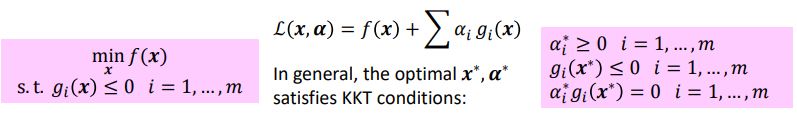
\includegraphics[width=1\textwidth]{fig/kkt1}
\label{fig:kkt1}
\end{figure}

\begin{figure}[!h]
\centering
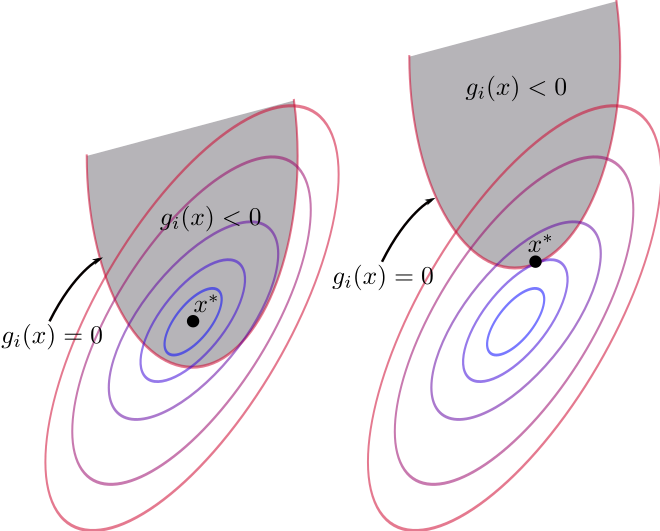
\includegraphics[width=0.8\textwidth]{fig/kkt2}
\label{fig:kkt2}
\end{figure}



\subsection{قیود غیرفعال:}
این قیودی است که بر حل بهینه مسئله تأثیر نمی‌گذارد. این قیود در سمت چپ اسلاید شما نمایش داده شده است. شرط برای قیود غیرفعال این است که در نقطه بهینه 
$(x^*)$ برابر با صفر نباشد، که به صورت ریاضی به صورت 
$g_i(x) \neq 0$
نمایش داده می‌شود. در نمودار، نقطه بهینه 
$(x^*)$
در داخل منطقه مجاز اما نه بر روی مرز تعریف شده توسط قیود قرار دارد، و ضریب لاگرانژ مربوطه $(α)$ برابر با صفر است.
$$y^{(n)} (w^Tx^{(n)} + w_0) > 1$$
$$\Rightarrow \alpha_n = 0 ,x^{(n)}$$
بردار پشتیبان نیست  . 


\subsection{قیود فعال:}
 این قیودی است که بر حل بهینه مسئله تأثیر مستقیم دارد. این قیود در سمت راست اسلاید شما نمایش داده شده است. برای قیود فعال، شرط این است که در نقطه بهینه 
$(x^*)$
برابر با صفر باشد، که به صورت ریاضی به صورت 
$(g_i(x) = 0)$ نمایش داده می‌شود. 
اینجا، نقطه بهینه 
$(x^*)$ 
بر روی مرز منطقه مجاز قرار دارد، که لبه تعریف شده توسط قیود است.
$$y^{(n)} (w^Tx^{(n)} + w_0) = 1$$

نقاطی که روی مارجین می افتند برای ما قیود فعال هستند که می توانند جای بهینه را عوض کنند . (همانطور که در فرمول مشخص است )

\begin{figure}[!h]
\centering
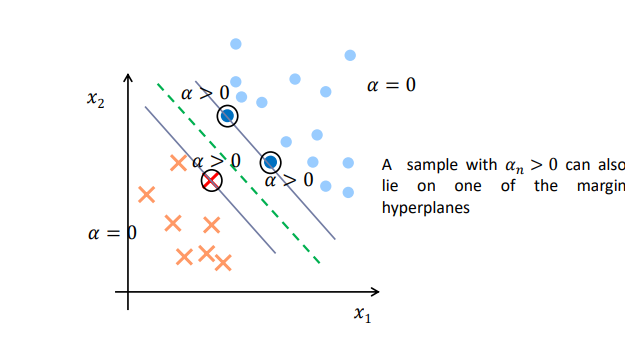
\includegraphics[width=0.8\textwidth]{fig/active.png}

\label{fig:active}
\end{figure}


$(SVs) = {x^{(n)} | \alpha_n > 0 }$
این بدان معنی است که یک بردار پشتیبان یک نقطه داده
$x^{(n)}$
است که ضریب لاگرانژ مربوطه برای آن بزرگتر از صفر است.

جهت ابر صفحه (مرز تصمیم) را می توان تنها بر اساس بردارهای پشتیبانی تعیین کرد. این به این دلیل است که بردارهای پشتیبان، نقاط داده ای هستند که نزدیک ترین نقطه به ابر صفحه قرار دارند و بیشترین تأثیر را در جهت آن دارند.


جهت ابرصفحه $W$ را می توان با استفاده از فرمول زیر محاسبه کرد:

$$w = \sum_{\alpha_n > 0 } \alpha_n y^{(n)} x^{(n)}$$


پس از حل مسئله برنامه نویسی درجه دوم (QP) برای یافتن ضرایب لاگرانژ، می توانیم بردار وزن را با استفاده از فرمول زیر پیدا کنیم:

$$w = \sum_{n=1}^{N} \alpha_n y^{(n)} x^{(n)}$$

هر یک از نمونه هایی که دارای
$\alpha_s > 0$
هستند در حاشیه قرار می گیرند
، به این معنی که آنها به ابرصفحه نزدیک ترین هستند. بنابراین، ما می‌توانیم از هر یک از این $SV$
ها برای حل
$w_0$
استفاده کنیم.

$$y(s)(\mathbf{w}^T \mathbf{x}^(s) + w_0) = 1$$
$$\Rightarrow w_0 = y^{(s)} - \mathbf{w}^T \mathbf{x}^{(s)}$$

\subsection{طبقه بندی نمونه های جدید}

هنگام طبقه‌بندی یک نمونه جدید، $SVM$ با حاشیه سخت از فرمول زیر استفاده می‌کند:

$$ \hat{y} = sign(w_0 + w^T x) $$
این نشان دهنده تابع تصمیم گیری یک 
$SVM$
است. برچسب پیش بینی شده 
$(\hat{y})$
را محاسبه می کند.

$$ \hat{y} = sign\left(w_0 + \left(\sum_{a_n > 0} a_n y^{(n)} x^{(n)}\right)^T x\right) $$


تابع تصمیم‌گیری به شکل گسترش یافتهبه صورت بالا است ،  مجموع بر روی همه بردارهای پشتیبان (نمونه‌هایی که$a_n > 0$) اجرا می‌شود.


$$ \hat{y} = sign\left(y^{(s)} - w_0 -\sum_{a_n > 0} a_n y^{(n)} (x^{(n)})^T x^{(s)}\right) +\sum_{a_n > 0} a_n y^{(n)} (x^{(n)})^T x $$



با جابجایی و کم و زیاد کردن واریانس کرنل گوشی ،مرز های ما بیشتر و بیشتر جابجا می شوند و اورفیت ایجاد می کنند  و دور هر دیتای ترین جمع و غیر خطی می شوند .

\begin{latin}
    $$
\max_{\alpha} \left( \sum_{n=1}^{N} \alpha_n - \frac{1}{2} \sum_{n=1}^{N} \sum_{m=1}^{N} \alpha_n \alpha_m y^{(n)} y^{(m)} \left( x^{(n)} \right)^T x^{(m)} \right)
$$
Subject to the constraints:
$$
\sum_{n=1}^{N} \quad \alpha_n y^{(n)} = 0
$$
and
$$
\alpha_n \geq 0 \quad \text{for } n = 1, \ldots, N
$$
\end{latin}

\section{ماشین بردار پشتیبان در مسائل خطی تفکیک ناپذیر($Soft-margin\:SVM$)
}
در بسیاری از مسائل دنیای واقعی، داده‌ها نمی‌توانند به طور کامل توسط یک مرز خطی جدا شوند. تقریبا جداپذیری خطی به داده‌هایی اشاره دارد که تقریباً می‌توانند توسط یک مرز خطی جدا شوند اما ممکن است چند نمونه به اشتباه طبقه‌بندی شده یا درون حاشیه قرار گیرند.
گاهی داده ها انقدر تمیز نیستند و ممکن است داده ها با آنکه به صورت خطی جداپذیر هستند، ولیدر هم رفته اند و کاملا تفکیک شده نباشند.
برای همچین حالاتی از
$Soft-margin\:SVM$
استفاده می کنیم .
\subsection{مفهوم حاشیه نرم}
هدف: حداکثر کردن حاشیه در حالی که اجازه می‌دهد برخی نقاط در طرف اشتباه حاشیه یا حتی اشتباه طبقه‌بندی شوند. متغیرهای شل \((\xi_i)\) برای هر نقطه داده برای اندازه‌گیری درجه اشتباه طبقه‌بندی یا نقض حاشیه معرفی شده‌اند.
\subsection{
کمینه کردن تعداد نقاط طبقه‌بندی شده اشتباه: }
ایده‌آل این است که یک $SVM$ تمام نقاط آموزشی را به طور کامل طبقه‌بندی کند. با این حال، این همیشه ممکن نیست، به ویژه با داده‌های پر سر و صدا. هدف کمینه کردن این طبقه‌بندی‌های اشتباه است.

در این حالت ما اجازه میدهیم برخی از داده ها در آموزش دچار خطا بشوند .

$SVM$
با حاشیه نرم یک متغیر اسلک 
$(slack\:variable) ( \xi )$ 
را برای هر نقطه داده معرفی می‌کند تا اجازه دهد برخی از طبقه‌بندی‌های اشتباه وجود داشته باشند. هدف یافتن تعادل بین حداکثر کردن حاشیه (فاصله بین صفحه جداکننده و نزدیک‌ترین نقاط داده از هر کلاس) و کمینه کردن مجموع این متغیرهای اسلک است که نمایانگر جریمه کلی برای هر گونه طبقه‌بندی اشتباه است.
\begin{latin}
    $$
\min_{w, b, \xi} \frac{1}{2} || w ||^2 + C \sum_{i=1}^{n} \xi_i
$$
Subject to the constraints:
$$
y^{(n)} (w^T x^{(n)} + w_0) \geq 1 - \xi_i \quad \text{and} \quad \xi_i \geq 0 \quad n = 1, \cdot , N
$$
\end{latin}

\begin{figure}[!h]
\centering
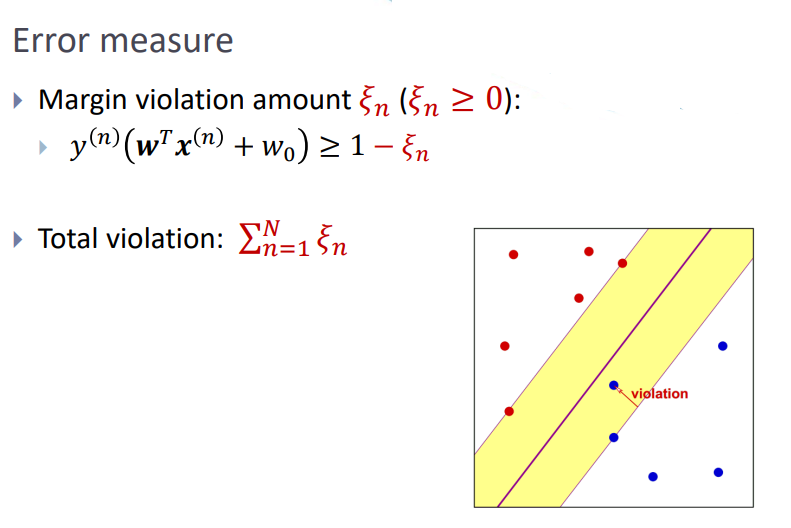
\includegraphics[width=0.8\textwidth]{fig/soft margin svm.png}

\label{fig:soft}
\end{figure}

\begin{figure}[!h]
\centering
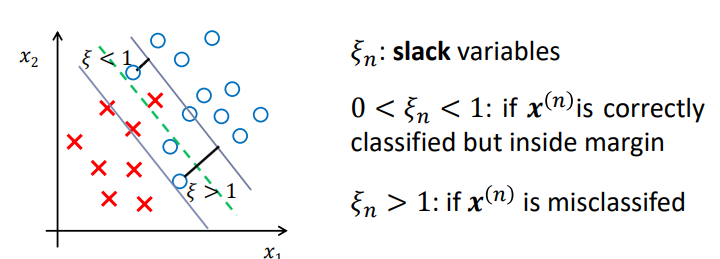
\includegraphics[width=0.8\textwidth]{fig/slack.png}

\label{fig:slack}
\end{figure}
دو دسته قید داریم
یکی مانند قبل و دیگری روی اسلک ها .

لاگرانژ روشی برای یافتن ماکزیمم و مینیمم های محلی یک تابع تحت قیود تساوی است، یعنی حداکثر $f(x,y)$ تحت قید $g(x,y)=c$. توابع $f(\cdot)$ و $g(\cdot)$ باید دارای مشتقات جزئی اول پیوسته باشند.

لگرانژیان، نمایش داده شده با $\mathcal{L}(x, y, \lambda)$, با ترکیب تابع هدف $f(x, y)$ و تابع قید $g(x, y)$ به همراه ضریب لاگرانژ $\lambda$ به دست می آید که می تواند مثبت یا منفی باشد. به طور ریاضی، $\mathcal{L}(x, y, \lambda) = f(x, y) + \lambda(g(x, y)-c)$.

اگر $f(x_0, y_0)$ ماکزیمم تابع $f(x, y)$ برای مسئله اصلی تحت قید باشد، سپس وجود دارد $\lambda$ به گونه ای که $(x_0, y_0, \lambda_0)$ یک نقطه ایستایی برای تابع لاگرانژ است (بنابراین $\partial \mathcal{L}/\partial x = \partial \mathcal{L}/\partial y = 0$).

تابع لاگرانژین را تشکیل میدهیم : 
$$
\mathcal{L}(w,w_{0},\xi,\alpha,\beta) = \frac{1}{2}||w||^{2}+C\sum_{n=1}^{N}\overline{\xi}_{n} + \\
\sum_{n=1}^{N}\alpha_{n}(1-\xi_{n}-y^{(n)}(w^{T}x^{(n)}+w_{0}))- \\
\sum_{n=1}^{N}\beta_{n}\xi_{n}
$$



\begin{equation}
\begin{aligned}
& \underset{\alpha}{max}
& & \sum_{n=1}^{N} \alpha_n - \frac{1}{2} \sum_{n=1}^{N} \sum_{m=1}^{N} 
  \alpha_n \alpha_m y^{(n)} y^{(m)} (x^{(n)})^T x^{(m)} \\
& s.t.
& & 0 \leq \alpha_n \leq C, \quad n = 1,\ldots,N \\
&&& 0 = \sum_{n=1}^N y^{(n)}\alpha_n
\end{aligned}
\end{equation}


 پس از حل مسئله درجه دوم بالا، $w$ به صورت زیر پیدا می شود:
$$w = \sum_{n=1}^{N}\alpha_n y^{(n)} x^{(n)} $$
\textbf{
شرایط کاروش-کان-تاکر $(KKT)$
}


شرایط $KKT$ مجموعه‌ای از شرایط ریاضی هستند که به ما کمک می‌کنند تا تعیین کنیم آیا یک راه‌حل برای یک مسئله بهینه‌سازی، بهینه است یا خیر. این شرایط ضروری هستند، به این معنا که اگر یک راه‌حل شرایط $KKT$ را برآورده کند، آنگاه می‌تواند یک راه‌حل بهینه باشد، اما ممکن است تنها راه‌حل بهینه نباشد.

شرایط $KKT$ به مسائل بهینه‌سازی که دارای یک تابع هدف و مجموعه‌ای از محدودیت‌ها هستند اعمال می‌شوند. تابع هدف، تابعی است که می‌خواهیم آن را کمینه یا بیشینه کنیم، و محدودیت‌ها شرایطی هستند که راه‌حل ما باید آن‌ها را برآورده کند.

در زمینه ماشین‌های بردار پشتیبان $(SVM)$، شرایط $KKT$ برای یافتن مقادیر بهینه وزن‌ها، بایاس، و ضرایب لاگرانژ که مرز تصمیم‌گیری $SVM$ را تعریف می‌کنند، استفاده می‌شود.


شرایط $KKT$ برای مسئله دوگان $SVM$ شامل موارد زیر است:

\begin{itemize}
    \item عدم منفی بودن ضرایب لاگرانژ: $\alpha_i \geq 0$ برای همه $i$.
    \item شرط حاشیه: $y^{(n)} (w^{*T}x^{(n)}+w_{0}^{*}) \geq 1 - \xi_n^*$ برای همه $n$. این شرط اطمینان می‌دهد که نقاط داده روی حاشیه دارای حاشیه تابعی حداقل 1 هستند.
    \item مکمل اسلک: $\alpha_i^* (1 - y^{(n)} ({w^{*}}^{T}x^{(n)}+w_{0}^{*}) - \xi_n^*) = 0$ برای همه $n$. این شرط اطمینان می‌دهد که یا ضریب لاگرانژ $\alpha_i^*$ صفر است یا محدودیت $y^{(n)} (w^{*T}x^{(n)}+w_{0}^{*}) \geq 1 - \xi_n^*$ به صورت مساوی برآورده شده است.
    \item عدم منفی بودن متغیرهای اسلک: $\xi_n \geq 0$ برای همه $n$. متغیرهای اسلک میزان مجاز نقض محدودیت حاشیه را اندازه‌گیری می‌کنند.
    \item عدم وجود شکاف دوگان: $\xi_n \beta_n = 0$ برای همه $n$. این شرط اطمینان می‌دهد که شکاف دوگان بین توابع هدف اولیه و دوگان مسئله بهینه‌سازی $SVM$ وجود ندارد.
\end{itemize}

\begin{frame}
\frametitle{\textbf{$SVM$ با حاشیه نرم: بردارهای پشتیبان}}

\begin{itemize}
    \item بردارهای پشتیبان نقاط داده آموزشی هستند که مرز تصمیم‌گیری (فراصفحه) $SVM$ را تعریف می‌کنند.
    
    \item دو نوع بردار پشتیبان وجود دارد که با مقدار ضریب لاگرانژ $\alpha_n$ مشخص می‌شوند:
    
        \begin{itemize}
           \item[1]  \textbf{بردارهای پشتیبان حاشیه:} این‌ها نقاط داده‌ای هستند که دقیقا روی حاشیه در اطراف مرز تصمیم‌گیری قرار دارند. این‌ها دارای $0 < \alpha_n < C$ هستند.
            
                \begin{itemize}
                    \item معادله $y^{(n)}(w^{T}x^{(n)} + w_{0}) = 1$ برای این بردارهای پشتیبان برقرار است، که به این معناست که این‌ها به درستی طبقه‌بندی شده‌اند و روی حاشیه قرار دارند.
                    
                    \item آن‌ها با $(\xi_n = 0)$ نمایش داده می‌شوند زیرا متغیر اسلک $\xi_n$ برای این نقاط صفر است.
                \end{itemize}
                
            \item[2]  \textbf{بردارهای پشتیبان غیر حاشیه $non-margin support vector$:} این‌ها نقاط داده‌ای هستند که در طرف اشتباه حاشیه یا داخل حاشیه قرار دارند. این‌ها دارای $\alpha_n = C$ هستند.
            
                \begin{itemize}
                    \item معادله $y^{(n)}(w^{T}x^{(n)} + w_{0}) < 1$ برای این بردارهای پشتیبان برقرار است، که به این معناست که این‌ها یا به اشتباه طبقه‌بندی شده‌اند یا به درستی طبقه‌بندی شده‌اند اما در داخل حاشیه قرار دارند.
                    
                    \item آن‌ها با $(\xi_n > 0)$ نمایش داده می‌شوند زیرا متغیر اسلک $\xi_n$ برای این نقاط بزرگتر از صفر است.
                    
                    \item معادله $C - \alpha_n - \beta_n = 0$ نیز برای این بردارهای پشتیبان صدق می‌کند.
                \end{itemize}
        \end{itemize}
    \end{itemize}

به طور کلی، بردارهای پشتیبان حاشیه عرض حاشیه را تعریف می‌کنند، در حالی که بردارهای پشتیبان غیر حاشیه اجازه می‌دهند که برخی از طبقه‌بندی‌ها اشتباه باشد اما بر اساس پارامتر هزینه $C$ جریمه می‌شوند. پارامتر هزینه $C$ تعادلی بین حداکثرسازی حاشیه و اجازه دادن به برخی اشتباهات طبقه‌بندی را کنترل می‌کند.

\end{frame}


تصاویر نمونه‌ای از یک ماشین بردار پشتیبان ($SVM$) را با استفاده از هسته گاوسی ($RBF$) برای طبقه‌بندی نشان می‌دهد که مرز تصمیم و نواحی حاشیه را نشان می‌دهد.


\begin{figure}[!h]
\centering
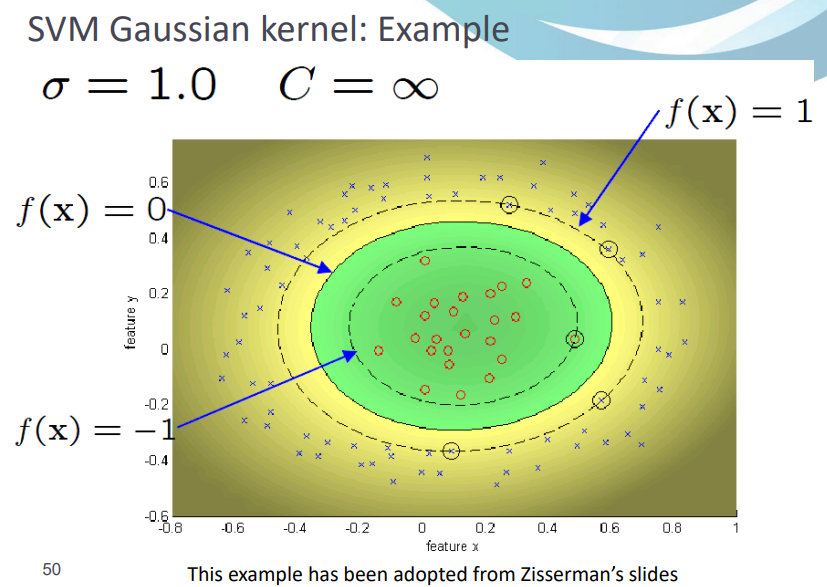
\includegraphics[width=0.8\textwidth]{fig/example 1.png}

\label{fig:kkt2}
\end{figure}

\begin{figure}[!h]
\centering
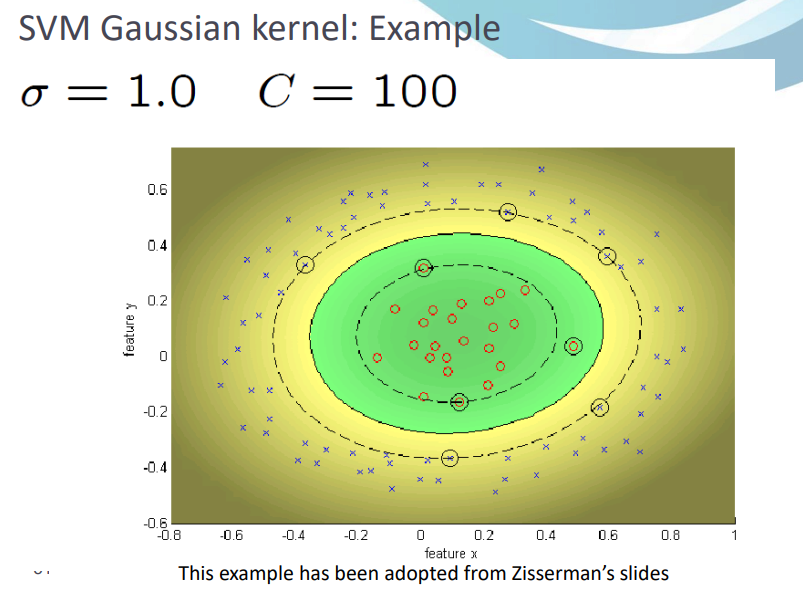
\includegraphics[width=0.8\textwidth]{fig/example 2.png}

\label{fig:kkt2}
\end{figure}

\begin{figure}[!h]
\centering
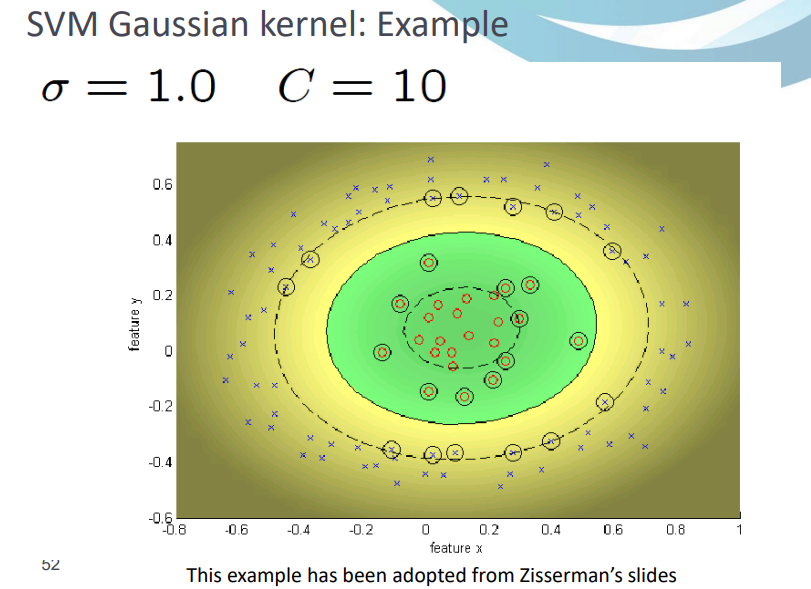
\includegraphics[width=0.8\textwidth]{fig/example 3.png}

\label{fig:kkt2}
\end{figure}

\begin{figure}[!h]
\centering
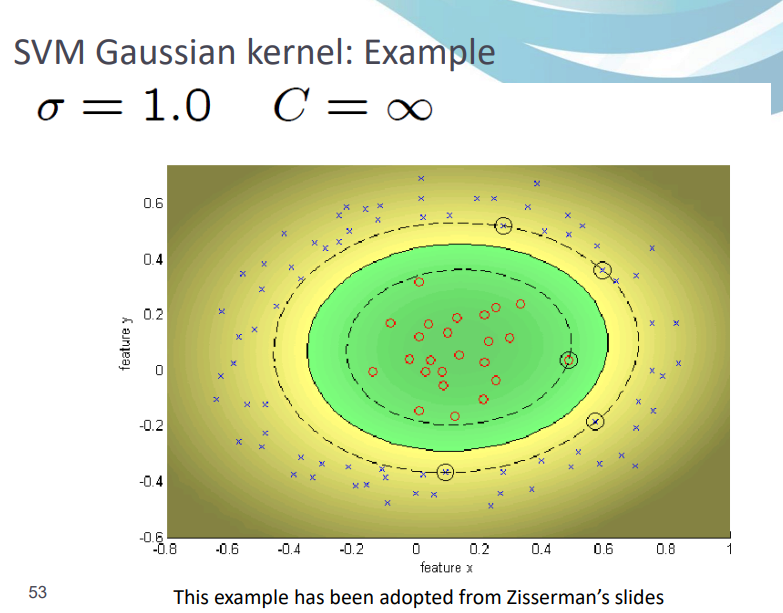
\includegraphics[width=0.8\textwidth]{fig/example 4.png}

\label{fig:kkt2}
\end{figure}

\begin{figure}[!h]
\centering
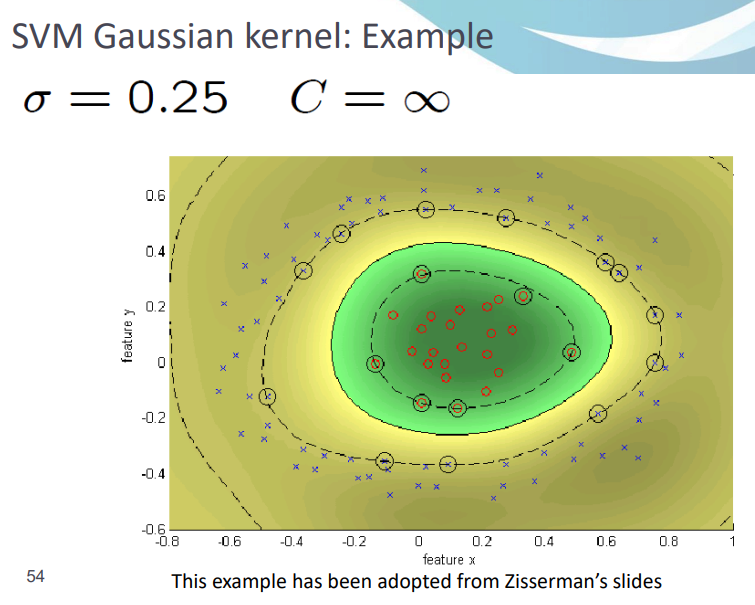
\includegraphics[width=0.8\textwidth]{fig/example 5.png}

\label{fig:kkt2}
\end{figure}

\begin{figure}[!h]
\centering
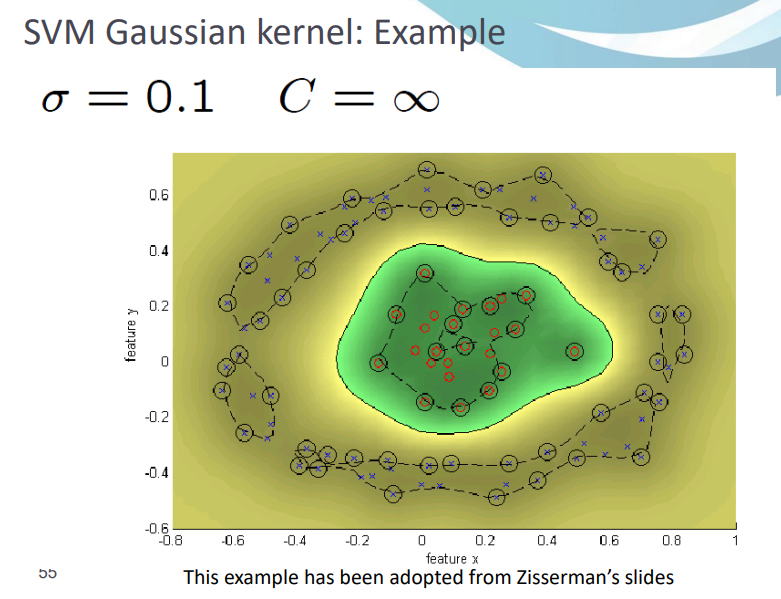
\includegraphics[width=0.8\textwidth]{fig/example 6.png}

\label{fig:kkt2}
\end{figure}
















\end{document}